\graphicspath{{_example/}}

\noindent
\textit{Just a few random pieces of text (latex) I wrote when I was still a student.}

\section{The importance of political behaviour}

\todo{Create an introduction}

\begin{quote}
\textit{The most serious political problems tend to arise over the collective production of goods that are also collectively consumed.} \citep[p. 34]{laver}
\end{quote}

\noindent
Rational individuals do not contribute to collective goods. They rather take a free ride, reaping the collective benefits without costs because they can not be excluded from a public good. If all individuals in the group are rational, then no one will contribute to the public good, and the realisation of the collective good will be hopeless. This collective action problem is best illustrated in the story of the "Tragedy of the Commons". A bunch of farmers have a common ground where sheep can pasture. If too many sheep graze, than the pasture will become over-grazed. But each individual farmer should add a few extra sheep on the pasture to maximize his profit, because the disadvantages from overgrazing will be shared by all. It is easy to see how this works out without some Hobbesian outsider who enforces rules to protect the pasture. \citep[p. 36, 48-50]{laver}

\ldots

Voter turnout of young adults is often low. \citet{plutzer} offers a developmental framework to understand turnout. In short, he distinguishes two kinds of citizens: habitual voters and habitual nonvoters. Both display inertia: becoming a voter needs some trigger, and vice versa. Education is an important tool to transform nonvoters in voters. \citeauthor{plutzer} regards age and development (education) as starting variables. Becoming a civic active citizen is a path-dependent process. One starts as a young nonvoter, and peer groups consists of other nonvoters. As one ages, one gets educated, married, a home owner and so on, one gets more incentives to vote and one gets more political knowledge. Once the inertia is overcome, a nonvoter becomes a voter and often (thanks to inertia) does not change back. The speed of this development can be increased by better political education and more participation to social groups and associations.

Cited: \cite{laver,plutzer}

\section{subfig}

\begin{figure}[h]
	\centering
	\subfloat[gebit foto 1]{
		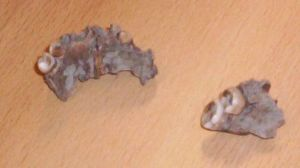
\includegraphics[scale=0.7]{gebit1.jpg}
	}
	\qquad
	\subfloat[gebit foto 2]{
		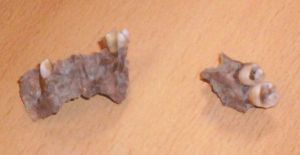
\includegraphics[scale=0.7]{gebit2.jpg}
	}
	\caption{Maxilla.}
	\label{fig:sk3_gebitten}
\end{figure}

Hier heeft \cite{laver} niets mee van doen.

\section{wrapfig}

\begin{wrapfigure}{R}{0pt}
	\centering
	%\begin{center}
		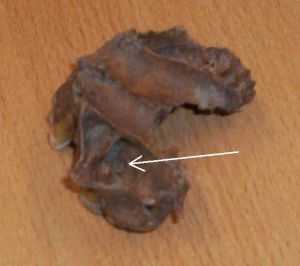
\includegraphics[width=0.6\textwidth]{fistel1.jpg}
	%\end{center}
	\caption{Fistel naar de sinus maxillaris.}
	\label{fig:fistel}
\end{wrapfigure}

\lipsum[1-3]

\section{Formatting}

Gebruik \emph{emph} en niet \emph{textit} omdat \emph{textit} niet kan nesten.
Bovendien is \emph{emph} semantisch en kan de opmaak ervan nog gewijzigd worden.
Zie ook \url{http://tex.stackexchange.com/questions/1980/emph-or-textit}

\begin{textbox}{Dit is een tekstbox}
\label{text:somename}
The actual text comes here.

Do you like it?
\end{textbox}

\subsection{Litagures -- try copy and paste}

ff fi fj fl ffi ffl ffj

\subsection{font stuff}

\sout{strikethrough},
\uwave{underwave},
\underline{underline},
\textcolor{red}{red},
\textcolor{OrangeRed}{OrangeRed},
\textsc{SmallCaps},
\texttt{TypeWriter},
\textit{Italics},
\textsl{Slanted},
\textbf{Bold},
\emph{Emphasis}

\subsection{unicode}

Does this work? Also copying and pasting to a text editor?

02 - comma's are `nice' \\
03 - euro € \\
04 - often used @ ! ( { [ ] } ) ~ \\
05 - commercial © ® ™ \\
06 - special ‘’‚‛“”„ comma \\
07 - funny ☺☻☼♠♣♥♦♫ \\
08 - gender ♂♀ \\
09 - math ≈≠≡≤√≥⅔₧ \\
10 - western ßæçèéëîñõø \\
11 - pi π \\
99 - runes ᚱᚢᚾᛖᛋ

Runes with the specific Hnias font, method 1 (newfontface):

\newfontface{\runes}{Hnias}
{\runes ᚱᚢᚾᛖᛋ}

Runes with the specific Hnias font, method 2 (xetex only):

%% XETEX Only!!
%% custom font, using a .ttf or .otf file
\setmainfont[Path=_example/]{Hnias31_runes.ttf}
%% set back to main font as specified in font_xetex.tex
ᚱᚢᚾᛖᛋ
\setmainfont{Linux Libertine O}

\section{Lijstjes}

\subsection{enumerate}

Bij de wervelkolom zijn diverse aandoeningen aanwezig:
\begin{enumerate}[I.] % I --> roman numbers, see formatting.tex in _PKG
\item Scoliose is vooral lumbaal goed zichtbaar bij de overgang naar het sacrum.
\item De spondylolyse op wervel L3 is terug te voeren op een mechanisch trauma. De wervelboog is afgebroken door teveel aanspanning (overbelasting) van de rugspieren. Hetzelfde euvel is ook bekend bij eskimo's die in kayaks hun rugspieren flink gebruiken, en bij mensen aan het begin van de vorige eeuw die tewerkgesteld werden en plots zware lichamelijke arbeid moesten verrichten waar ze niet aan gewend waren.
\item Beginnende DDD is vooral hoog lumbaal en laag thoracaal zichtbaar. Er zijn forse Schmorlse noduli.
\end{enumerate}

\subsection{description}

\begin{description}[style=sameline,leftmargin=3cm] % the options are from the enumitem package
\item[Data users] such as the departments of radiology and psychiatry.
\item[ADICT] the IT department of the AMC, also responsible for the IT security policy of the AMC.
\item[Ethical Board] of the AMC which might offer opinions and facts about patient privacy
\end{description}

\subsection{itemize}

Using interviews has also a number of drawbacks:
\begin{itemize}
\item The interpretation of interviews is very subjective.
\item Subjects could be restricted because anonymization is nearly impossible.
\item Organizational (political) sensitivities could be triggered.
\end{itemize}

\subsection{table}

\begin{table}\footnotesize
	\centering
	\begin{tabularx}{\textwidth}{ X l l l l l l l }
		&\rotatebox{90}{Jean Herveg}	&\rotatebox{90}{Corette Ploem}	&\rotatebox{90}{Heleen Dupuis}	&\rotatebox{90}{Bart van der Sloot}	&\rotatebox{90}{Beer Franken}	&\rotatebox{90}{Neugrid}	&\rotatebox{90}{MEAN}\\
	\hline \\
	Is informed consent needed?	&+	&+	&+	&+[4]	&+	&+	&+\\
	 $\backslash$-- If yes, must it be written consent?	&?	&+	&?	&?	&?	&+	&+\\
	 $\backslash$-- If yes, must it be specific for each research?	&+	&-[2]	&+	&+	&?	&+	&+\\
	Is genetic data medical data or (also) identifiable and personal data?	&+	&+	&+	&+	&+	&+	&+\\
	Is it allowed to use distributed computing?	&+[1]	&?	&+	&?	&?	&+	&+\\
	 $\backslash$-- If it is, is it also allowed to process facial images and genetic data?	&?	&?	&-	&-	&-	&+	&-\\
	Must a contract between all involved into the distributed resources be present?	&?	&?	&+	&?	&+	&?	&+\\
	Could distributed computing be used for patient care such as diagnosis or treatment (non-research)?	&?	&?	&+[3]	&+		&-&?	&?\\
	\hline \\
	\end{tabularx}
	\noindent
	+ = yes, - = no, ? = unknown or missing
	\begin{enumerate}
		\item yes, but maybe current security measures are not strong enough
		\item a broad consent for the use of tissue is practical, but for each specific research a new ethical review is necessary
		\item yes, but only if all data is encrypted
		\item but informed consent is outdated and problematic (see interview)
	\end{enumerate}
	\caption{Opinions of experts}
	\label{expertopinions}
\end{table}

\begin{table}[H]
	\centering
	\begin{tabular}{ l l l }
		Fruit	&Price	&Taste\\
		\hline \\
		Oragne	&5	&Nice\\
		Apple	&6	&Good\\
	\end{tabular}
	\caption{Fruits.}
	\label{fruits}
\end{table}

\section{Equations}

Math modes

$a+b=\int_{\xi}^{\theta} f(x)\,dx$

$a+b=∫_ξ^θ f(x)\,dx$

\section{Author}

\begin{wrapfigure}{l}{0pt}
	%\begin{center}
		
\includegraphics[width=30pt]{evert.jpg}
	%\end{center}
\end{wrapfigure}

\paragraph{Evert Mouw}
\textit{studeerde politicologie en medische informatica}\\
Email: post@evert.net

\paragraph{Barge's Anthropologica} houdt zich bezig met wetenschappelijk onderzoek en onderwijs op het gebied van fysische antropologie. Het centrum is verbonden aan het Leids Universitair Medisch Centrum. Dit verslag is tot stand gekomen als onderdeel van een studieopdracht tijdens de zomercursus voor studenten in 2007. Meer informatie over het centrum is te vinden op \url{http://www.bargesanthropologica.nl/}.
